% !Mode:: "TeX:UTF-8"
%!TEX program  = xelatex

% \documentclass{cumcmthesis}
\documentclass[withoutpreface,bwprint]{cumcmthesis} %去掉封面与编号页

\usepackage{url}
\title{Analysis and Forecast of the Pet Industry through Mathematical Models}
% \tihao{A}
% \baominghao{4321}
% \schoolname{XX大学}
% \membera{小米}
% \memberb{向左}
% \memberc{哈哈}
% \supervisor{老师}
% \yearinput{2017}
% \monthinput{08}
% \dayinput{22}
\usepackage{ctex}
\usepackage{setspace}
\usepackage{lipsum}
\usepackage{graphicx}%插入图片
\usepackage{cite}
\usepackage{hyperref}
\begin{document}
\bibliographystyle{plain}% 参考文献引用格式
 \maketitle
 \begin{abstract}
    The pet industry has witnessed significant growth globally, driven by increasing disposable income and the rising popularity of pet companionship. This paper explores the development and forecasting of the pet industry using mathematical models, with a focus on China's market trends and global demands. Through the application of ARIMA, polynomial interpolation, and multiple linear regression, this study analyzes the past five years of the pet industry in China, forecasting its development over the next three years. Additionally, global trends and the impact of economic factors, such as tariffs, on the pet food industry are considered. The results provide valuable insights for strategic recommendations and sustainable development in the pet industry.
    
% \uwave{关注我们的微信公众号}:
\begin{figure}[htbp]
	\centering
	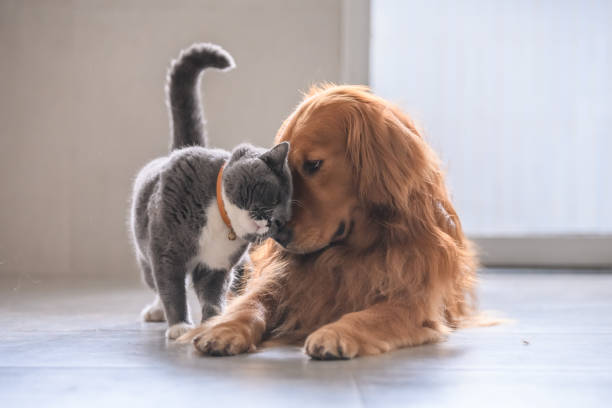
\includegraphics[scale=2.5]{istockphoto-992637094-612x612}
	\caption{British short hair cat and golden retriever stock photo\cite{1}}
\end{figure}
% \centerline{
\includegraphics[width=5cm]{gongzhonghao}}
% \caption{this is Ali}

\keywords{Pet Industry, Mathematical Models, ARIMA, Polynomial Interpolation, Multiple Linear Regression, Forecasting, Market Analysis, Economic Factors, Pet Food, Sustainable Development}
\end{abstract}

%目录
\tableofcontents

\section{Problem Restatement}

This problem requires analyzing and forecasting the development trends of the pet industry in China and globally, with a focus on the pet food market. The analysis should combine historical data and additional data collected, building mathematical models for prediction. The specific tasks are as follows:
\subsection{Question 1: Development of China's Pet Industry}

\subsubsection{Objective}
Analyze the development of China's pet industry over the past five years by different pet types (e.g., cats, dogs, etc.).
\subsubsection{Factors}
Look into economic factors, societal trends, and market changes (e.g., income growth, changes in pet ownership behavior, product innovations).
\subsubsection{Modeling Task}
Develop a mathematical model to predict the growth and development of China's pet industry for the next three years.
\subsection{Question 2: Global Pet Industry Development}
\subsubsection{Objective}
Analyze the development of the global pet industry, focusing on different regions (e.g., Europe, America, China).
\subsubsection{Factors}
Global pet food demand and market characteristics by pet type.
\subsubsection{Modeling Task}
Create a model to forecast the global demand for pet food over the next three years, based on data provided.
\subsection{Question 3: China's Pet Food Industry}
\subsubsection{Objective}
Analyze the development of China's pet food industry, specifically its production and export values.
\subsubsection{Factors}
The trend in China's pet food production and exports, factoring in the global demand for pet food.
\subsubsection{Modeling Task}
Predict China's pet food production and export trends over the next three years.
\subsection{Question 4: Impact of Foreign Economic Policies}
\subsubsection{Objective}
Analyze the impact of foreign economic policies on China's pet industry, focusing on trade barriers and tariffs.
\subsubsection{Factors}
Quantitative modeling of the effects of changes in tariffs and other foreign policies on China's pet food industry.
\subsubsection{Modeling Task}
Develop a model to assess the impact of these policies on China's pet food industry and suggest strategies for sustainable development.
\section{Model Assumptions}

\begin{itemize}
    \item Stability of human society
    \item Exclusion of potential future policies related to pets
    \item Ignoring changes in pet population due to major incidents
\end{itemize}

\section{Symbol Explanation}
\begin{center}
\begin{tabular}{cc}
 \hline
 \makebox[0.3\textwidth][c]{Symbol}	&  \makebox[0.4\textwidth][c]{Meaning} \\ \hline
 $\ln$ 	    & Logarithmic Function \\ \hline
 $\sum$ 	    & Sum  \\ \hline
 $M$	    & Million  \\ \hline
 $N$	    & Number  \\ \hline
\end{tabular}
\end{center}

\section{Analysis}

\subsection{Question 1 Analysis}
The task first requires us to analyze the development trends of the pet industry in China by categorizing pets 
and identifying the factors that influence the growth of the pet industry.
We should begin by analyzing the data.
\par The following data is provided to us in the problem.
\begin{table}[!htbp]
    \caption{2019-2023 Number of Pet Cats and Dogs in China (in 10,000s)} \centering
    \begin{tabular}{cccccc}
    \toprule[1.5pt]
    Pets/Years & 2023 & 2022 & 2021 & 2020 & 2019 \\
    \midrule[1pt]
    Cat & 6980 & 6536 & 5806 & 4862 & 4412 \\
    Dog & 5175 & 5119 & 5429 & 5222 & 5503 \\
    \bottomrule[1.5pt]
    \end{tabular}
    \end{table}
\par Plot the trend of changes in the pet population in China. 
A line chart is more intuitive than a table.
Thanks to the help of python, we can easily plot the line chart by the following code.
\begin{lstlisting}[language=python]
import pandas as pd
import matplotlib.pyplot as plt
with open('data_1.txt', 'r') as file:
    lines = file.readlines()
years = lines[0].split()[1:]
cat_data = lines[1].split()[1:]
dog_data = lines[2].split()[1:]
years = [int(year) for year in years]
cat_data = [int(num) for num in cat_data]
dog_data = [int(num) for num in dog_data]
plt.figure(figsize=(10, 6))
plt.plot(years, cat_data, marker='o', label='Cat')
plt.plot(years, dog_data, marker='o', label='Dog')
plt.xlabel('Year')
plt.ylabel('Number')
plt.title('Cat and Dog Numbers Over Years')
plt.legend()
plt.grid(True)
plt.show()
\end{lstlisting}
\begin{figure}[htbp]
	\centering
	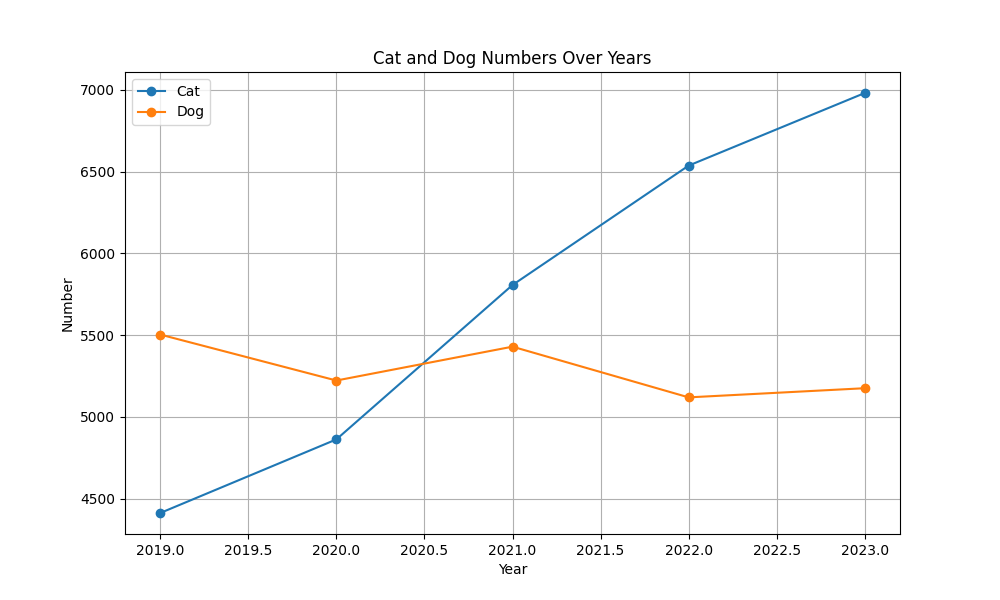
\includegraphics[scale=0.6]{Figure_2}
	\caption{Number of Cat and Dog in China from 2019 to 2023}
\end{figure}
\par 图像中看出,猫上升,狗数量几乎不变,猫的这种增长很有可能是由于人们生活水平的提高,越来越多的人开始养宠物。
所以,GDP很可能是影响宠物数量的一个因素。通过查阅资料,我们发现,GDP的增长率与宠物数量的增长率有很强的相关性。
因此,为了预测宠物数量的增长,我们可以使用GDP的增长率来预测宠物数量的增长率。
而对于狗,我们没有找到GDP增长率与狗数量增长率的直接关系。但是我们可以肯定,宠物经济的发展会带动宠物数量的增长。
故宠物经济很可能也与宠物数量的增长有很强的相关性。


\par We aim to predict the data for the next three years based on the data from the previous five years, starting with polynomial interpolation.
\begin{definition}[Polynomial Interpolation]
Given \( n+1 \) points, polynomial interpolation refers to finding a polynomial such that it satisfies the condition
\[
    P(x) = a_n x^n + a_{n-1} x^{n-1} + \dots + a_1 x + a_0
\]
That is, the image of the polynomial \( y = P(x) \) must pass through the given \( n+1 \) points \( (x_i, y_i) \).
\end{definition}

问题流程图:
\begin{figure}[!h]
\centering
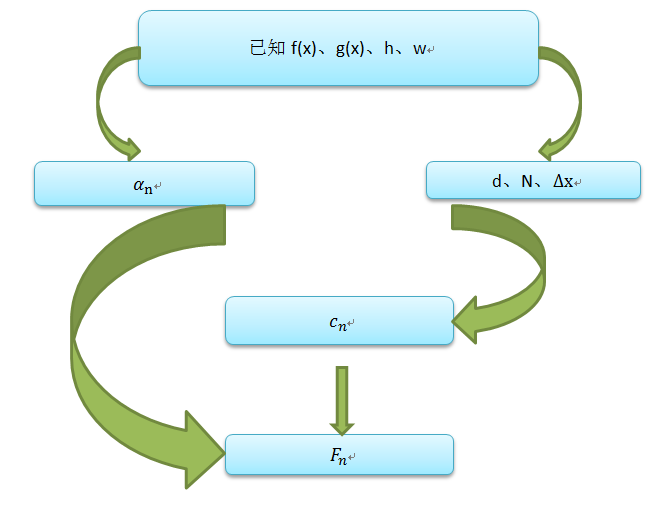
\includegraphics[width=.6\textwidth]{1.png}
\caption{问题三流程图}
\end{figure}

\section{绘制普通三线表格}
表格应具有三线表格式,因此常用 booktabs宏包,其标准格式如表~\ref{tab001}~所示。
\begin{table}[!htbp]
\caption{标准三线表格}\label{tab001} \centering
\begin{tabular}{ccccc}
\toprule[1.5pt]
$D$(in) & $P_u$(lbs) & $u_u$(in) & $\beta$ & $G_f$(psi.in)\\
\midrule[1pt]
 5 & 269.8 & 0.000674 & 1.79 & 0.04089\\
10 & 421.0 & 0.001035 & 3.59 & 0.04089\\
20 & 640.2 & 0.001565 & 7.18 & 0.04089\\
\bottomrule[1.5pt]
\end{tabular}
\end{table}

其绘制表格的代码及其说明如下。
\begin{tcode}
\begin{table}[!htbp]
\caption[标签名]{中文标题}
\begin{tabular}{cc...c}
\toprule[1.5pt]
表头第1个格   & 表头第2个格   & ... & 表头第n个格  \\
\midrule[1pt]
表中数据(1,1) & 表中数据(1,2) & ... & 表中数据(1,n)\\
表中数据(2,1) & 表中数据(2,2) & ... & 表中数据(2,n)\\
...................................................\\
表中数据(m,1) & 表中数据(m,2) & ... & 表中数据(m,n)\\
\bottomrule[1.5pt]
\end{tabular}
\end{table}
\end{tcode}

\bigskip
table环境是一个将表格嵌入文本的浮动环境。
tabular环境的必选参数由每列对应一个格式字符所组成:c表示居中,l表示左对齐,r表示右对齐,其总
个数应与表的列数相同。此外,\verb|@{文本}|可以出现在任意两个上述的列格式之间,其中的文本将被插入每一行
的同一位置。表格的各行以\verb|\\|分隔,同一行的各列则以\&分隔。
\verb|\toprule|、\verb|\midrule|和\verb|\bottomrule|三个命令是由booktabs宏包提供的,其
中\verb|\toprule|和\verb|\bottomrule|分别用来绘制表格的第一条(表格最顶部)和第三条(表格最底部)水平线,
\verb|\midrule|用来绘制第二条(表头之下)水平线,且第一条和第三条水平线的线宽为1.5pt,第二条水平线的线宽为1pt。
引用方法:“如表~\verb|\ref{标签名}|~所示”。


%参考文献
\begin{thebibliography}{9}%宽度9
 \bibitem{bib:one} ....
 \bibitem{bib:two} ....
\end{thebibliography}

\newpage
%附录
\begin{appendices}
\section{排队算法--matlab 源程序}
\begin{lstlisting}[language=matlab]
kk=2;[mdd,ndd]=size(dd);
while ~isempty(V)
[tmpd,j]=min(W(i,V));tmpj=V(j);
for k=2:ndd
[tmp1,jj]=min(dd(1,k)+W(dd(2,k),V));
tmp2=V(jj);tt(k-1,:)=[tmp1,tmp2,jj];
end
tmp=[tmpd,tmpj,j;tt];[tmp3,tmp4]=min(tmp(:,1));
if tmp3==tmpd, ss(1:2,kk)=[i;tmp(tmp4,2)];
else,tmp5=find(ss(:,tmp4)~=0);tmp6=length(tmp5);
if dd(2,tmp4)==ss(tmp6,tmp4)
ss(1:tmp6+1,kk)=[ss(tmp5,tmp4);tmp(tmp4,2)];
else, ss(1:3,kk)=[i;dd(2,tmp4);tmp(tmp4,2)];
end;end
dd=[dd,[tmp3;tmp(tmp4,2)]];V(tmp(tmp4,3))=[];
[mdd,ndd]=size(dd);kk=kk+1;
end; S=ss; D=dd(1,:);
 \end{lstlisting}
 \section{规划解决程序--lingo源代码}
\begin{lstlisting}[language=c]
kk=2;
[mdd,ndd]=size(dd);
while ~isempty(V)
    [tmpd,j]=min(W(i,V));tmpj=V(j);
for k=2:ndd
    [tmp1,jj]=min(dd(1,k)+W(dd(2,k),V));
    tmp2=V(jj);tt(k-1,:)=[tmp1,tmp2,jj];
end
    tmp=[tmpd,tmpj,j;tt];[tmp3,tmp4]=min(tmp(:,1));
if tmp3==tmpd, ss(1:2,kk)=[i;tmp(tmp4,2)];
else,tmp5=find(ss(:,tmp4)~=0);tmp6=length(tmp5);
if dd(2,tmp4)==ss(tmp6,tmp4)
    ss(1:tmp6+1,kk)=[ss(tmp5,tmp4);tmp(tmp4,2)];
else, ss(1:3,kk)=[i;dd(2,tmp4);tmp(tmp4,2)];
end;
end
    dd=[dd,[tmp3;tmp(tmp4,2)]];V(tmp(tmp4,3))=[];
    [mdd,ndd]=size(dd);
    kk=kk+1;
end;
S=ss;
D=dd(1,:);
 \end{lstlisting}
\end{appendices}
\bibliography{books}
\end{document} 